%!TEX program = xelatex 
\documentclass{standalone}%opcao draft remove os links
\usepackage{amssymb,amsmath,amsfonts,amsthm,amstext,pxfonts}
\usepackage{graphicx}
\usepackage[usenames,dvipsnames]{xcolor}
\usepackage{subfigure}
\usepackage{tikz,tikz-3dplot,tkz-euclide,circuitikz,siunitx,pstricks-add,pst-coil,pst-3dplot}
\usepackage{pst-plot,pst-func,pst-eucl,pst-solides3d}
\usetkzobj{all}
\usetikzlibrary{scopes}
\usetikzlibrary{through}
\usetikzlibrary{lindenmayersystems}
\usetikzlibrary[shadings]
\usetikzlibrary{arrows}
\usetikzlibrary{intersections,positioning}

\newcommand{\norm}[1]{\left\Vert{#1}\right\Vert}
\newcommand{\eq}{=}

\begin{document}
    \pagenumbering{gobble}
    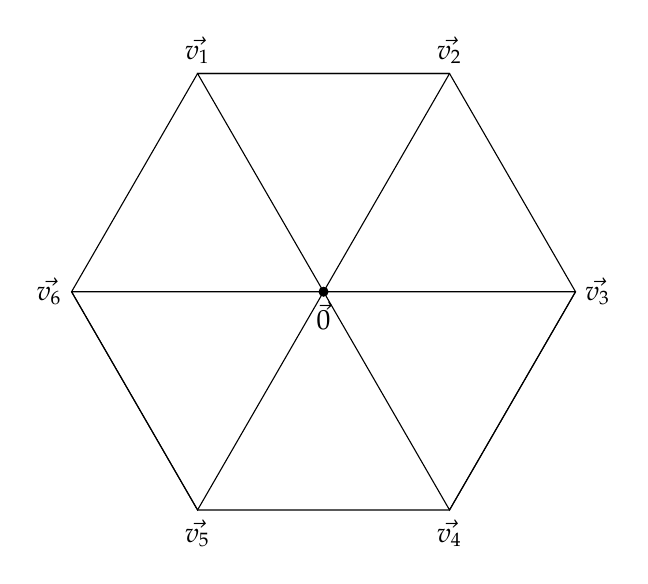
\begin{tikzpicture}[scale=4,cap=round,>=latex]
      % Radius of regular polygons
      \newdimen\R
      \R=0.8cm
      \coordinate (center) at (0,0);
      \draw (0:\R)
            \foreach \x in {60,120,...,360} {  -- (\x:\R) }
              -- cycle (300:\R) node[below] {$\vec{v_4}$}
              -- cycle (240:\R) node[below] {$\vec{v_5}$}
              -- cycle (180:\R) node[left] {$\vec{v_6}$}
              -- cycle (120:\R) node[above] {$\vec{v_1}$}
              -- cycle (60:\R) node[above] {$\vec{v_2}$}
              -- cycle (0:\R) node[right] {$\vec{v_3}$};
      \draw { (60:\R) -- (120:\R) -- (center) -- (60:\R) };
      \draw { (180:\R) -- (240:\R) -- (center) -- (180:\R) };
      \draw { (0:\R) -- (300:\R) -- (center) -- (0:\R) };
      \filldraw[black] (0:0cm) circle(0.4pt);
      \coordinate [label=-90:$\vec{0}$](o) at (0,0);
    \end{tikzpicture}
\end{document}